\documentclass{standalone}
\usepackage{tikz}
\usetikzlibrary{patterns, positioning}
\usepackage[sfdefault]{ClearSans} %% option 'sfdefault' activates Clear Sans as the default text font
\usepackage[T1]{fontenc}

\begin{document}
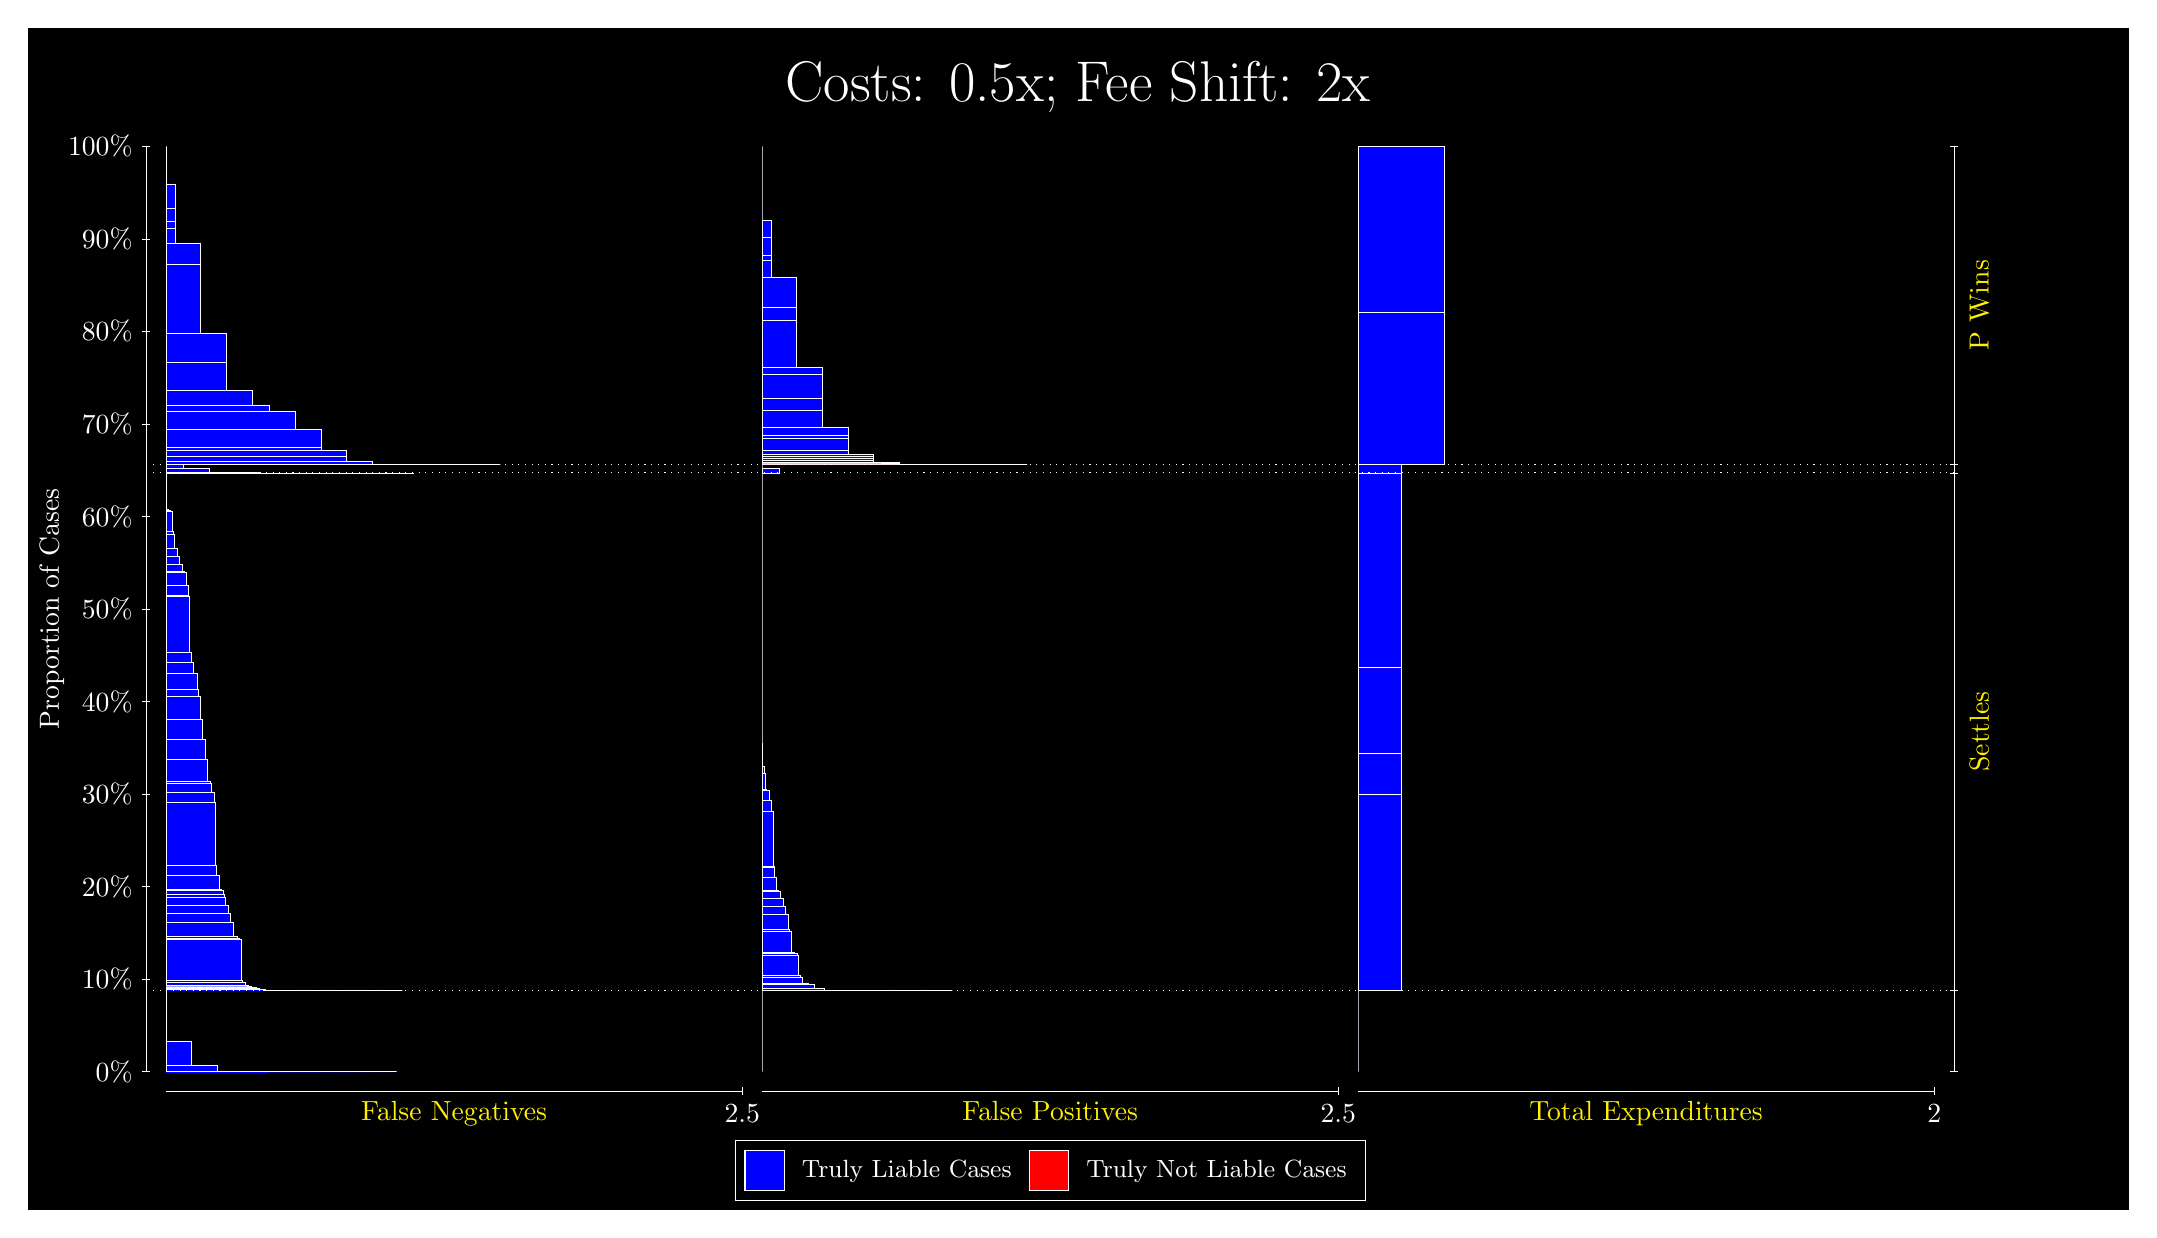
\begin{tikzpicture}
\draw[fill=black] (0,0) rectangle (26.667,15);
\draw[text=white] (0,13.5) rectangle (26.667,15) node[midway] {\huge Costs: 0.5x; Fee Shift: 2x};
\draw[white, very thin] (1.5,1.75) -- (1.5,13.5);
\node[rotate=90, text=white, anchor=center] at (0.3, 7.625) {Proportion of Cases};
\draw[white, very thin] (1.45,1.75) -- (1.55,1.75);
\node[text=white, anchor=east] at (1.45, 1.75) {0\%};
\draw[white, very thin] (1.45,2.925) -- (1.55,2.925);
\node[text=white, anchor=east] at (1.45, 2.925) {10\%};
\draw[white, very thin] (1.45,4.1) -- (1.55,4.1);
\node[text=white, anchor=east] at (1.45, 4.1) {20\%};
\draw[white, very thin] (1.45,5.275) -- (1.55,5.275);
\node[text=white, anchor=east] at (1.45, 5.275) {30\%};
\draw[white, very thin] (1.45,6.45) -- (1.55,6.45);
\node[text=white, anchor=east] at (1.45, 6.45) {40\%};
\draw[white, very thin] (1.45,7.625) -- (1.55,7.625);
\node[text=white, anchor=east] at (1.45, 7.625) {50\%};
\draw[white, very thin] (1.45,8.8) -- (1.55,8.8);
\node[text=white, anchor=east] at (1.45, 8.8) {60\%};
\draw[white, very thin] (1.45,9.975) -- (1.55,9.975);
\node[text=white, anchor=east] at (1.45, 9.975) {70\%};
\draw[white, very thin] (1.45,11.15) -- (1.55,11.15);
\node[text=white, anchor=east] at (1.45, 11.15) {80\%};
\draw[white, very thin] (1.45,12.325) -- (1.55,12.325);
\node[text=white, anchor=east] at (1.45, 12.325) {90\%};
\draw[white, very thin] (1.45,13.5) -- (1.55,13.5);
\node[text=white, anchor=east] at (1.45, 13.5) {100\%};

\draw[white, very thin] (24.457,1.75) -- (24.457,13.5);
\draw[white, very thin] (24.407,1.75) -- (24.507,1.75);
\node[anchor=west] at (24.407, 1.75) {};
\draw[white, very thin] (24.407,2.784) -- (24.507,2.784);
\node[anchor=west] at (24.407, 2.784) {};
\draw[white, very thin] (24.407,9.3537) -- (24.507,9.3537);
\node[anchor=west] at (24.407, 9.3537) {};
\draw[white, very thin] (24.407,9.4621) -- (24.507,9.4621);
\node[anchor=west] at (24.407, 9.4621) {};
\draw[white, very thin] (24.407,13.5) -- (24.507,13.5);
\node[anchor=west] at (24.407, 13.5) {};

\draw[white, very thin, fill=blue] (1.75,1.75) rectangle (4.6775,1.75);
\draw[white, very thin, fill=blue] (1.75,1.75) rectangle (4.3523,1.75);
\draw[white, very thin, fill=blue] (1.75,1.75) rectangle (4.027,1.75);
\draw[white, very thin, fill=blue] (1.75,1.75) rectangle (3.7017,1.75);
\draw[white, very thin, fill=blue] (1.75,1.75) rectangle (3.3764,1.75);
\draw[white, very thin, fill=blue] (1.75,1.75) rectangle (3.0511,1.7503);
\draw[white, very thin, fill=blue] (1.75,1.7503) rectangle (2.7258,1.7573);
\draw[white, very thin, fill=blue] (1.75,1.7573) rectangle (2.4006,1.8289);
\draw[white, very thin, fill=blue] (1.75,1.8289) rectangle (2.0753,2.1333);
\draw[white, very thin, fill=red] (1.75,2.1333) rectangle (1.75,2.1333);
\draw[white, very thin, fill=blue] (1.75,2.1333) rectangle (1.75,2.784);
\draw[white, very thin, fill=blue] (1.75,2.784) rectangle (4.7507,2.784);
\draw[white, very thin, fill=blue] (1.75,2.784) rectangle (4.6044,2.784);
\draw[white, very thin, fill=blue] (1.75,2.784) rectangle (4.458,2.784);
\draw[white, very thin, fill=blue] (1.75,2.784) rectangle (4.4255,2.784);
\draw[white, very thin, fill=blue] (1.75,2.784) rectangle (4.3116,2.784);
\draw[white, very thin, fill=blue] (1.75,2.784) rectangle (4.2791,2.784);
\draw[white, very thin, fill=blue] (1.75,2.784) rectangle (4.1652,2.784);
\draw[white, very thin, fill=blue] (1.75,2.784) rectangle (4.1327,2.784);
\draw[white, very thin, fill=blue] (1.75,2.784) rectangle (4.1002,2.784);
\draw[white, very thin, fill=blue] (1.75,2.784) rectangle (4.0188,2.784);
\draw[white, very thin, fill=blue] (1.75,2.784) rectangle (3.9863,2.784);
\draw[white, very thin, fill=blue] (1.75,2.784) rectangle (3.9538,2.784);
\draw[white, very thin, fill=blue] (1.75,2.784) rectangle (3.8725,2.784);
\draw[white, very thin, fill=blue] (1.75,2.784) rectangle (3.8399,2.784);
\draw[white, very thin, fill=blue] (1.75,2.784) rectangle (3.8074,2.784);
\draw[white, very thin, fill=blue] (1.75,2.784) rectangle (3.7749,2.784);
\draw[white, very thin, fill=blue] (1.75,2.784) rectangle (3.7261,2.784);
\draw[white, very thin, fill=blue] (1.75,2.784) rectangle (3.6936,2.784);
\draw[white, very thin, fill=blue] (1.75,2.784) rectangle (3.661,2.784);
\draw[white, very thin, fill=blue] (1.75,2.784) rectangle (3.6285,2.784);
\draw[white, very thin, fill=blue] (1.75,2.784) rectangle (3.5797,2.784);
\draw[white, very thin, fill=blue] (1.75,2.784) rectangle (3.5472,2.784);
\draw[white, very thin, fill=blue] (1.75,2.784) rectangle (3.5147,2.784);
\draw[white, very thin, fill=blue] (1.75,2.784) rectangle (3.4821,2.784);
\draw[white, very thin, fill=blue] (1.75,2.784) rectangle (3.4496,2.784);
\draw[white, very thin, fill=blue] (1.75,2.784) rectangle (3.4333,2.784);
\draw[white, very thin, fill=blue] (1.75,2.784) rectangle (3.4008,2.784);
\draw[white, very thin, fill=blue] (1.75,2.784) rectangle (3.3683,2.784);
\draw[white, very thin, fill=blue] (1.75,2.784) rectangle (3.3358,2.784);
\draw[white, very thin, fill=blue] (1.75,2.784) rectangle (3.3032,2.784);
\draw[white, very thin, fill=blue] (1.75,2.784) rectangle (3.287,2.784);
\draw[white, very thin, fill=blue] (1.75,2.784) rectangle (3.2544,2.7846);
\draw[white, very thin, fill=blue] (1.75,2.7846) rectangle (3.2219,2.7847);
\draw[white, very thin, fill=blue] (1.75,2.7847) rectangle (3.1894,2.7848);
\draw[white, very thin, fill=blue] (1.75,2.7848) rectangle (3.1568,2.7848);
\draw[white, very thin, fill=blue] (1.75,2.7848) rectangle (3.1406,2.7852);
\draw[white, very thin, fill=blue] (1.75,2.7852) rectangle (3.1243,2.7852);
\draw[white, very thin, fill=blue] (1.75,2.7852) rectangle (3.1081,2.7852);
\draw[white, very thin, fill=blue] (1.75,2.7852) rectangle (3.0755,2.7874);
\draw[white, very thin, fill=blue] (1.75,2.7874) rectangle (3.043,2.788);
\draw[white, very thin, fill=blue] (1.75,2.788) rectangle (3.0105,2.7885);
\draw[white, very thin, fill=blue] (1.75,2.7885) rectangle (2.9779,2.7888);
\draw[white, very thin, fill=blue] (1.75,2.7888) rectangle (2.9617,2.7891);
\draw[white, very thin, fill=blue] (1.75,2.7891) rectangle (2.9292,2.8109);
\draw[white, very thin, fill=blue] (1.75,2.8109) rectangle (2.8966,2.8196);
\draw[white, very thin, fill=blue] (1.75,2.8196) rectangle (2.8641,2.8258);
\draw[white, very thin, fill=blue] (1.75,2.8258) rectangle (2.8316,2.8317);
\draw[white, very thin, fill=blue] (1.75,2.8317) rectangle (2.8153,2.8387);
\draw[white, very thin, fill=blue] (1.75,2.8387) rectangle (2.799,2.8413);
\draw[white, very thin, fill=blue] (1.75,2.8413) rectangle (2.7828,2.8415);
\draw[white, very thin, fill=blue] (1.75,2.8415) rectangle (2.7502,2.886);
\draw[white, very thin, fill=blue] (1.75,2.886) rectangle (2.7177,2.9076);
\draw[white, very thin, fill=blue] (1.75,2.9076) rectangle (2.7015,3.4268);
\draw[white, very thin, fill=blue] (1.75,3.4268) rectangle (2.6852,3.4465);
\draw[white, very thin, fill=blue] (1.75,3.4465) rectangle (2.6527,3.4621);
\draw[white, very thin, fill=blue] (1.75,3.4621) rectangle (2.6364,3.467);
\draw[white, very thin, fill=blue] (1.75,3.467) rectangle (2.6039,3.6446);
\draw[white, very thin, fill=blue] (1.75,3.6446) rectangle (2.5713,3.7577);
\draw[white, very thin, fill=blue] (1.75,3.7577) rectangle (2.5388,3.8559);
\draw[white, very thin, fill=blue] (1.75,3.8559) rectangle (2.5063,3.9569);
\draw[white, very thin, fill=blue] (1.75,3.9569) rectangle (2.49,4.0063);
\draw[white, very thin, fill=blue] (1.75,4.0063) rectangle (2.4738,4.0565);
\draw[white, very thin, fill=blue] (1.75,4.0565) rectangle (2.4575,4.0587);
\draw[white, very thin, fill=blue] (1.75,4.0587) rectangle (2.425,4.2361);
\draw[white, very thin, fill=blue] (1.75,4.2361) rectangle (2.3924,4.3668);
\draw[white, very thin, fill=blue] (1.75,4.3668) rectangle (2.3762,5.1678);
\draw[white, very thin, fill=blue] (1.75,5.1678) rectangle (2.3599,5.2956);
\draw[white, very thin, fill=blue] (1.75,5.2956) rectangle (2.3274,5.4085);
\draw[white, very thin, fill=blue] (1.75,5.4085) rectangle (2.3111,5.4304);
\draw[white, very thin, fill=blue] (1.75,5.4304) rectangle (2.2786,5.712);
\draw[white, very thin, fill=blue] (1.75,5.712) rectangle (2.2461,5.9701);
\draw[white, very thin, fill=blue] (1.75,5.9701) rectangle (2.2135,6.2181);
\draw[white, very thin, fill=blue] (1.75,6.2181) rectangle (2.181,6.5152);
\draw[white, very thin, fill=blue] (1.75,6.5152) rectangle (2.1647,6.6028);
\draw[white, very thin, fill=blue] (1.75,6.6028) rectangle (2.1485,6.808);
\draw[white, very thin, fill=blue] (1.75,6.808) rectangle (2.1322,6.8128);
\draw[white, very thin, fill=blue] (1.75,6.8128) rectangle (2.0997,6.9489);
\draw[white, very thin, fill=blue] (1.75,6.9489) rectangle (2.0672,7.0774);
\draw[white, very thin, fill=blue] (1.75,7.0774) rectangle (2.0509,7.7838);
\draw[white, very thin, fill=blue] (1.75,7.7838) rectangle (2.0346,7.7982);
\draw[white, very thin, fill=blue] (1.75,7.7982) rectangle (2.0346,7.9203);
\draw[white, very thin, fill=blue] (1.75,7.9203) rectangle (2.0021,8.0855);
\draw[white, very thin, fill=blue] (1.75,8.0855) rectangle (1.9858,8.1045);
\draw[white, very thin, fill=blue] (1.75,8.1045) rectangle (1.9533,8.1908);
\draw[white, very thin, fill=blue] (1.75,8.1908) rectangle (1.9208,8.2895);
\draw[white, very thin, fill=blue] (1.75,8.2895) rectangle (1.8882,8.3911);
\draw[white, very thin, fill=blue] (1.75,8.3911) rectangle (1.8557,8.5775);
\draw[white, very thin, fill=blue] (1.75,8.5775) rectangle (1.8395,8.6075);
\draw[white, very thin, fill=blue] (1.75,8.6075) rectangle (1.8232,8.8697);
\draw[white, very thin, fill=blue] (1.75,8.8697) rectangle (1.8069,8.8715);
\draw[white, very thin, fill=blue] (1.75,8.8715) rectangle (1.7744,8.8904);
\draw[white, very thin, fill=red] (1.75,8.8904) rectangle (1.75,8.8904);
\draw[white, very thin, fill=blue] (1.75,8.8904) rectangle (1.75,9.3537);
\draw[white, very thin, fill=blue] (1.75,9.3537) rectangle (4.8971,9.3537);
\draw[white, very thin, fill=blue] (1.75,9.3537) rectangle (4.5718,9.3537);
\draw[white, very thin, fill=blue] (1.75,9.3537) rectangle (4.2465,9.3537);
\draw[white, very thin, fill=blue] (1.75,9.3537) rectangle (3.9213,9.3537);
\draw[white, very thin, fill=blue] (1.75,9.3537) rectangle (3.596,9.3537);
\draw[white, very thin, fill=blue] (1.75,9.3537) rectangle (3.2707,9.3537);
\draw[white, very thin, fill=blue] (1.75,9.3537) rectangle (2.9454,9.3542);
\draw[white, very thin, fill=blue] (1.75,9.3542) rectangle (2.6201,9.3647);
\draw[white, very thin, fill=blue] (1.75,9.3647) rectangle (2.2948,9.4075);
\draw[white, very thin, fill=blue] (1.75,9.4075) rectangle (1.9696,9.4621);
\draw[white, very thin, fill=red] (1.75,9.4621) rectangle (1.75,9.4621);
\draw[white, very thin, fill=blue] (1.75,9.4621) rectangle (5.9949,9.4621);
\draw[white, very thin, fill=blue] (1.75,9.4621) rectangle (5.6697,9.4621);
\draw[white, very thin, fill=blue] (1.75,9.4621) rectangle (5.3444,9.4621);
\draw[white, very thin, fill=blue] (1.75,9.4621) rectangle (5.3444,9.4621);
\draw[white, very thin, fill=blue] (1.75,9.4621) rectangle (5.0191,9.4624);
\draw[white, very thin, fill=blue] (1.75,9.4624) rectangle (4.7914,9.4624);
\draw[white, very thin, fill=blue] (1.75,9.4624) rectangle (4.6938,9.4661);
\draw[white, very thin, fill=blue] (1.75,9.4661) rectangle (4.4661,9.4661);
\draw[white, very thin, fill=blue] (1.75,9.4661) rectangle (4.4661,9.4661);
\draw[white, very thin, fill=blue] (1.75,9.4661) rectangle (4.3685,9.4947);
\draw[white, very thin, fill=blue] (1.75,9.4947) rectangle (4.1408,9.4947);
\draw[white, very thin, fill=blue] (1.75,9.4947) rectangle (4.0432,9.5674);
\draw[white, very thin, fill=blue] (1.75,9.5674) rectangle (4.0432,9.6347);
\draw[white, very thin, fill=blue] (1.75,9.6347) rectangle (3.8155,9.6347);
\draw[white, very thin, fill=blue] (1.75,9.6347) rectangle (3.8155,9.6347);
\draw[white, very thin, fill=blue] (1.75,9.6347) rectangle (3.718,9.6817);
\draw[white, very thin, fill=blue] (1.75,9.6817) rectangle (3.718,9.9062);
\draw[white, very thin, fill=blue] (1.75,9.9062) rectangle (3.4903,9.9063);
\draw[white, very thin, fill=blue] (1.75,9.9063) rectangle (3.3927,10.135);
\draw[white, very thin, fill=blue] (1.75,10.135) rectangle (3.3927,10.135);
\draw[white, very thin, fill=blue] (1.75,10.135) rectangle (3.165,10.137);
\draw[white, very thin, fill=blue] (1.75,10.137) rectangle (3.165,10.141);
\draw[white, very thin, fill=blue] (1.75,10.141) rectangle (3.0674,10.206);
\draw[white, very thin, fill=blue] (1.75,10.206) rectangle (2.8397,10.402);
\draw[white, very thin, fill=blue] (1.75,10.402) rectangle (2.7421,10.402);
\draw[white, very thin, fill=blue] (1.75,10.402) rectangle (2.7421,10.403);
\draw[white, very thin, fill=blue] (1.75,10.403) rectangle (2.7421,10.403);
\draw[white, very thin, fill=blue] (1.75,10.403) rectangle (2.5144,10.755);
\draw[white, very thin, fill=blue] (1.75,10.755) rectangle (2.5144,11.122);
\draw[white, very thin, fill=blue] (1.75,11.122) rectangle (2.4168,11.122);
\draw[white, very thin, fill=blue] (1.75,11.122) rectangle (2.4168,11.122);
\draw[white, very thin, fill=blue] (1.75,11.122) rectangle (2.1891,12.004);
\draw[white, very thin, fill=blue] (1.75,12.004) rectangle (2.1891,12.267);
\draw[white, very thin, fill=blue] (1.75,12.267) rectangle (2.0915,12.267);
\draw[white, very thin, fill=blue] (1.75,12.267) rectangle (2.0915,12.267);
\draw[white, very thin, fill=blue] (1.75,12.267) rectangle (1.8638,12.458);
\draw[white, very thin, fill=blue] (1.75,12.458) rectangle (1.8638,12.548);
\draw[white, very thin, fill=blue] (1.75,12.548) rectangle (1.8638,12.717);
\draw[white, very thin, fill=blue] (1.75,12.717) rectangle (1.8638,13.024);
\draw[white, very thin, fill=blue] (1.75,13.024) rectangle (1.7663,13.024);
\draw[white, very thin, fill=blue] (1.75,13.024) rectangle (1.7663,13.024);
\draw[white, very thin, fill=red] (1.75,13.024) rectangle (1.75,13.024);
\draw[white, very thin, fill=blue] (1.75,13.024) rectangle (1.75,13.5);
\draw[white, very thin, fill=red] (9.3189,1.75) rectangle (9.3189,1.75);
\draw[white, very thin, fill=blue] (9.3189,1.75) rectangle (9.3189,2.784);
\draw[white, very thin, fill=red] (9.3189,2.784) rectangle (11.734,2.784);
\draw[white, very thin, fill=blue] (9.3189,2.784) rectangle (11.734,2.784);
\draw[white, very thin, fill=blue] (9.3189,2.784) rectangle (11.409,2.784);
\draw[white, very thin, fill=red] (9.3189,2.784) rectangle (11.295,2.784);
\draw[white, very thin, fill=blue] (9.3189,2.784) rectangle (11.295,2.784);
\draw[white, very thin, fill=red] (9.3189,2.784) rectangle (11.149,2.784);
\draw[white, very thin, fill=blue] (9.3189,2.784) rectangle (11.149,2.784);
\draw[white, very thin, fill=blue] (9.3189,2.784) rectangle (11.084,2.784);
\draw[white, very thin, fill=red] (9.3189,2.784) rectangle (11.002,2.784);
\draw[white, very thin, fill=blue] (9.3189,2.784) rectangle (11.002,2.784);
\draw[white, very thin, fill=blue] (9.3189,2.784) rectangle (10.97,2.784);
\draw[white, very thin, fill=red] (9.3189,2.784) rectangle (10.856,2.784);
\draw[white, very thin, fill=blue] (9.3189,2.784) rectangle (10.856,2.784);
\draw[white, very thin, fill=blue] (9.3189,2.784) rectangle (10.823,2.784);
\draw[white, very thin, fill=blue] (9.3189,2.784) rectangle (10.758,2.784);
\draw[white, very thin, fill=red] (9.3189,2.784) rectangle (10.709,2.784);
\draw[white, very thin, fill=blue] (9.3189,2.784) rectangle (10.709,2.784);
\draw[white, very thin, fill=blue] (9.3189,2.784) rectangle (10.677,2.784);
\draw[white, very thin, fill=blue] (9.3189,2.784) rectangle (10.644,2.784);
\draw[white, very thin, fill=red] (9.3189,2.784) rectangle (10.563,2.784);
\draw[white, very thin, fill=blue] (9.3189,2.784) rectangle (10.563,2.784);
\draw[white, very thin, fill=blue] (9.3189,2.784) rectangle (10.531,2.784);
\draw[white, very thin, fill=blue] (9.3189,2.784) rectangle (10.498,2.784);
\draw[white, very thin, fill=blue] (9.3189,2.784) rectangle (10.433,2.7845);
\draw[white, very thin, fill=red] (9.3189,2.7845) rectangle (10.417,2.7845);
\draw[white, very thin, fill=blue] (9.3189,2.7845) rectangle (10.417,2.7845);
\draw[white, very thin, fill=blue] (9.3189,2.7845) rectangle (10.384,2.7845);
\draw[white, very thin, fill=blue] (9.3189,2.7845) rectangle (10.352,2.7845);
\draw[white, very thin, fill=blue] (9.3189,2.7845) rectangle (10.319,2.7845);
\draw[white, very thin, fill=red] (9.3189,2.7845) rectangle (10.27,2.7845);
\draw[white, very thin, fill=blue] (9.3189,2.7845) rectangle (10.27,2.7847);
\draw[white, very thin, fill=blue] (9.3189,2.7847) rectangle (10.238,2.7847);
\draw[white, very thin, fill=blue] (9.3189,2.7847) rectangle (10.205,2.7848);
\draw[white, very thin, fill=blue] (9.3189,2.7848) rectangle (10.173,2.7848);
\draw[white, very thin, fill=red] (9.3189,2.7848) rectangle (10.124,2.7848);
\draw[white, very thin, fill=blue] (9.3189,2.7848) rectangle (10.124,2.7863);
\draw[white, very thin, fill=red] (9.3189,2.7863) rectangle (10.124,2.7863);
\draw[white, very thin, fill=blue] (9.3189,2.7863) rectangle (10.124,2.7865);
\draw[white, very thin, fill=blue] (9.3189,2.7865) rectangle (10.108,2.8107);
\draw[white, very thin, fill=blue] (9.3189,2.8107) rectangle (10.091,2.8112);
\draw[white, very thin, fill=blue] (9.3189,2.8112) rectangle (10.059,2.8117);
\draw[white, very thin, fill=blue] (9.3189,2.8117) rectangle (10.026,2.8118);
\draw[white, very thin, fill=blue] (9.3189,2.8118) rectangle (9.9938,2.8136);
\draw[white, very thin, fill=red] (9.3189,2.8136) rectangle (9.9776,2.8136);
\draw[white, very thin, fill=blue] (9.3189,2.8136) rectangle (9.9776,2.8547);
\draw[white, very thin, fill=blue] (9.3189,2.8547) rectangle (9.945,2.8622);
\draw[white, very thin, fill=blue] (9.3189,2.8622) rectangle (9.9125,2.8684);
\draw[white, very thin, fill=blue] (9.3189,2.8684) rectangle (9.88,2.8732);
\draw[white, very thin, fill=blue] (9.3189,2.8732) rectangle (9.8475,2.876);
\draw[white, very thin, fill=red] (9.3189,2.876) rectangle (9.8312,2.876);
\draw[white, very thin, fill=blue] (9.3189,2.876) rectangle (9.8312,2.9507);
\draw[white, very thin, fill=blue] (9.3189,2.9507) rectangle (9.7987,2.9758);
\draw[white, very thin, fill=blue] (9.3189,2.9758) rectangle (9.7987,2.9784);
\draw[white, very thin, fill=blue] (9.3189,2.9784) rectangle (9.7824,3.2268);
\draw[white, very thin, fill=blue] (9.3189,3.2268) rectangle (9.7661,3.2473);
\draw[white, very thin, fill=blue] (9.3189,3.2473) rectangle (9.7336,3.2662);
\draw[white, very thin, fill=blue] (9.3189,3.2662) rectangle (9.7011,3.268);
\draw[white, very thin, fill=red] (9.3189,3.268) rectangle (9.6848,3.268);
\draw[white, very thin, fill=blue] (9.3189,3.268) rectangle (9.6848,3.5302);
\draw[white, very thin, fill=blue] (9.3189,3.5302) rectangle (9.6685,3.5603);
\draw[white, very thin, fill=blue] (9.3189,3.5603) rectangle (9.6523,3.7466);
\draw[white, very thin, fill=blue] (9.3189,3.7466) rectangle (9.6198,3.8482);
\draw[white, very thin, fill=blue] (9.3189,3.8482) rectangle (9.5872,3.9469);
\draw[white, very thin, fill=blue] (9.3189,3.9469) rectangle (9.5547,4.0332);
\draw[white, very thin, fill=blue] (9.3189,4.0332) rectangle (9.5222,4.0522);
\draw[white, very thin, fill=blue] (9.3189,4.0522) rectangle (9.5059,4.2174);
\draw[white, very thin, fill=blue] (9.3189,4.2174) rectangle (9.4734,4.3395);
\draw[white, very thin, fill=blue] (9.3189,4.3395) rectangle (9.4734,4.354);
\draw[white, very thin, fill=blue] (9.3189,4.354) rectangle (9.4571,5.0603);
\draw[white, very thin, fill=blue] (9.3189,5.0603) rectangle (9.4408,5.1889);
\draw[white, very thin, fill=blue] (9.3189,5.1889) rectangle (9.4083,5.3249);
\draw[white, very thin, fill=blue] (9.3189,5.3249) rectangle (9.3758,5.3297);
\draw[white, very thin, fill=blue] (9.3189,5.3297) rectangle (9.3595,5.5349);
\draw[white, very thin, fill=blue] (9.3189,5.5349) rectangle (9.3433,5.6225);
\draw[white, very thin, fill=blue] (9.3189,5.6225) rectangle (9.327,5.9196);
\draw[white, very thin, fill=blue] (9.3189,5.9196) rectangle (9.3189,9.3537);
\draw[white, very thin, fill=red] (9.3189,9.3537) rectangle (9.5384,9.3537);
\draw[white, very thin, fill=blue] (9.3189,9.3537) rectangle (9.5384,9.4083);
\draw[white, very thin, fill=blue] (9.3189,9.4083) rectangle (9.3189,9.4621);
\draw[white, very thin, fill=red] (9.3189,9.4621) rectangle (12.686,9.4621);
\draw[white, very thin, fill=blue] (9.3189,9.4621) rectangle (12.686,9.4621);
\draw[white, very thin, fill=red] (9.3189,9.4621) rectangle (12.36,9.4621);
\draw[white, very thin, fill=blue] (9.3189,9.4621) rectangle (12.36,9.4621);
\draw[white, very thin, fill=red] (9.3189,9.4621) rectangle (12.035,9.4621);
\draw[white, very thin, fill=blue] (9.3189,9.4621) rectangle (12.035,9.4621);
\draw[white, very thin, fill=blue] (9.3189,9.4621) rectangle (12.035,9.4621);
\draw[white, very thin, fill=blue] (9.3189,9.4621) rectangle (12.035,9.4621);
\draw[white, very thin, fill=red] (9.3189,9.4621) rectangle (11.71,9.4621);
\draw[white, very thin, fill=blue] (9.3189,9.4621) rectangle (11.71,9.4622);
\draw[white, very thin, fill=blue] (9.3189,9.4622) rectangle (11.71,9.4623);
\draw[white, very thin, fill=red] (9.3189,9.4623) rectangle (11.384,9.4623);
\draw[white, very thin, fill=blue] (9.3189,9.4623) rectangle (11.384,9.4629);
\draw[white, very thin, fill=blue] (9.3189,9.4629) rectangle (11.384,9.4643);
\draw[white, very thin, fill=blue] (9.3189,9.4643) rectangle (11.059,9.4703);
\draw[white, very thin, fill=red] (9.3189,9.4703) rectangle (11.059,9.4703);
\draw[white, very thin, fill=blue] (9.3189,9.4703) rectangle (11.059,9.4748);
\draw[white, very thin, fill=blue] (9.3189,9.4748) rectangle (11.059,9.4826);
\draw[white, very thin, fill=red] (9.3189,9.4826) rectangle (10.831,9.4826);
\draw[white, very thin, fill=blue] (9.3189,9.4826) rectangle (10.831,9.4826);
\draw[white, very thin, fill=blue] (9.3189,9.4826) rectangle (10.734,9.5137);
\draw[white, very thin, fill=blue] (9.3189,9.5137) rectangle (10.734,9.5405);
\draw[white, very thin, fill=red] (9.3189,9.5405) rectangle (10.734,9.5405);
\draw[white, very thin, fill=blue] (9.3189,9.5405) rectangle (10.734,9.5683);
\draw[white, very thin, fill=blue] (9.3189,9.5683) rectangle (10.734,9.5872);
\draw[white, very thin, fill=red] (9.3189,9.5872) rectangle (10.506,9.5872);
\draw[white, very thin, fill=blue] (9.3189,9.5872) rectangle (10.506,9.5872);
\draw[white, very thin, fill=blue] (9.3189,9.5872) rectangle (10.506,9.5872);
\draw[white, very thin, fill=blue] (9.3189,9.5872) rectangle (10.409,9.6344);
\draw[white, very thin, fill=red] (9.3189,9.6344) rectangle (10.409,9.6344);
\draw[white, very thin, fill=blue] (9.3189,9.6344) rectangle (10.409,9.7961);
\draw[white, very thin, fill=blue] (9.3189,9.7961) rectangle (10.409,9.8271);
\draw[white, very thin, fill=blue] (9.3189,9.8271) rectangle (10.409,9.9378);
\draw[white, very thin, fill=blue] (9.3189,9.9378) rectangle (10.181,9.9378);
\draw[white, very thin, fill=red] (9.3189,9.9378) rectangle (10.181,9.9378);
\draw[white, very thin, fill=blue] (9.3189,9.9378) rectangle (10.181,9.9378);
\draw[white, very thin, fill=blue] (9.3189,9.9378) rectangle (10.083,10.153);
\draw[white, very thin, fill=blue] (9.3189,10.153) rectangle (10.083,10.302);
\draw[white, very thin, fill=red] (9.3189,10.302) rectangle (10.083,10.302);
\draw[white, very thin, fill=blue] (9.3189,10.302) rectangle (10.083,10.609);
\draw[white, very thin, fill=blue] (9.3189,10.609) rectangle (10.083,10.695);
\draw[white, very thin, fill=blue] (9.3189,10.695) rectangle (9.8556,10.695);
\draw[white, very thin, fill=red] (9.3189,10.695) rectangle (9.8556,10.695);
\draw[white, very thin, fill=blue] (9.3189,10.695) rectangle (9.8556,10.695);
\draw[white, very thin, fill=blue] (9.3189,10.695) rectangle (9.8556,10.695);
\draw[white, very thin, fill=blue] (9.3189,10.695) rectangle (9.758,11.287);
\draw[white, very thin, fill=blue] (9.3189,11.287) rectangle (9.758,11.455);
\draw[white, very thin, fill=blue] (9.3189,11.455) rectangle (9.758,11.84);
\draw[white, very thin, fill=blue] (9.3189,11.84) rectangle (9.5303,11.84);
\draw[white, very thin, fill=red] (9.3189,11.84) rectangle (9.5303,11.84);
\draw[white, very thin, fill=blue] (9.3189,11.84) rectangle (9.5303,11.84);
\draw[white, very thin, fill=blue] (9.3189,11.84) rectangle (9.5303,11.84);
\draw[white, very thin, fill=blue] (9.3189,11.84) rectangle (9.4327,12.056);
\draw[white, very thin, fill=blue] (9.3189,12.056) rectangle (9.4327,12.112);
\draw[white, very thin, fill=blue] (9.3189,12.112) rectangle (9.4327,12.34);
\draw[white, very thin, fill=blue] (9.3189,12.34) rectangle (9.4327,12.559);
\draw[white, very thin, fill=red] (9.3189,12.559) rectangle (9.3189,12.559);
\draw[white, very thin, fill=blue] (9.3189,12.559) rectangle (9.3189,13.5);
\draw[white, very thin, fill=red] (16.888,1.75) rectangle (16.888,1.75);
\draw[white, very thin, fill=blue] (16.888,1.75) rectangle (16.888,2.784);
\draw[white, very thin, fill=red] (16.888,2.784) rectangle (17.437,2.784);
\draw[white, very thin, fill=blue] (16.888,2.784) rectangle (17.437,5.2657);
\draw[white, very thin, fill=red] (16.888,5.2657) rectangle (17.437,5.2657);
\draw[white, very thin, fill=blue] (16.888,5.2657) rectangle (17.437,5.7859);
\draw[white, very thin, fill=red] (16.888,5.7859) rectangle (17.437,5.7859);
\draw[white, very thin, fill=blue] (16.888,5.7859) rectangle (17.437,6.8778);
\draw[white, very thin, fill=red] (16.888,6.8778) rectangle (17.437,6.8778);
\draw[white, very thin, fill=blue] (16.888,6.8778) rectangle (17.437,9.3537);
\draw[white, very thin, fill=red] (16.888,9.3537) rectangle (17.437,9.3537);
\draw[white, very thin, fill=blue] (16.888,9.3537) rectangle (17.437,9.4621);
\draw[white, very thin, fill=red] (16.888,9.4621) rectangle (17.986,9.4621);
\draw[white, very thin, fill=blue] (16.888,9.4621) rectangle (17.986,11.393);
\draw[white, very thin, fill=red] (16.888,11.393) rectangle (17.986,11.393);
\draw[white, very thin, fill=blue] (16.888,11.393) rectangle (17.986,13.5);
\draw[white, dotted] (1.5,2.784) -- (24.457,2.784);
\draw[white, dotted] (1.5,9.3537) -- (24.457,9.3537);
\draw[white, dotted] (1.5,9.4621) -- (24.457,9.4621);
\draw[white, very thin] (1.75,1.5) -- (9.0689,1.5);
\node[text=yellow, anchor=north] at (5.4094, 1.5) {False Negatives};
\draw[white, very thin] (9.0689,1.45) -- (9.0689,1.55);
\node[text=white, anchor=north] at (9.0689, 1.45) {2.5};

\draw[white, very thin] (9.3189,1.5) -- (16.638,1.5);
\node[text=yellow, anchor=north] at (12.978, 1.5) {False Positives};
\draw[white, very thin] (16.638,1.45) -- (16.638,1.55);
\node[text=white, anchor=north] at (16.638, 1.45) {2.5};

\draw[white, very thin] (16.888,1.5) -- (24.207,1.5);
\node[text=yellow, anchor=north] at (20.547, 1.5) {Total Expenditures};
\draw[white, very thin] (24.207,1.45) -- (24.207,1.55);
\node[text=white, anchor=north] at (24.207, 1.45) {2};


\node[text=yellow, centered, rotate=90] at (24.777, 6.0689) {Settles};

\node[text=yellow, centered, rotate=90] at (24.777, 11.481) {P Wins};

\draw (12.978300999999998,1.5) node[draw=none] (baseCoordinate) {};
\begin{scope}[align=center]
        \matrix[scale=0.5, draw=white, below=0.5cm of baseCoordinate, nodes={draw}, column sep=0.1cm]{
            \node[rectangle, draw, minimum width=0.5cm, minimum height=0.5cm, fill=blue] {}; &
            \node[draw=none, font=\small, text=white] (B) {Truly Liable Cases}; &
            \node[rectangle, draw, minimum width=0.5cm, minimum height=0.5cm, fill=red] {}; &
            \node[draw=none, font=\small, text=white] (B) {Truly Not Liable Cases}; \\
            };
\end{scope}

\end{tikzpicture}
\end{document}